\chapter{Ergebnisse der Evaluation}
\label{chap4}

Dieses Kapitel diskutiert die vier in Kapitel 3 definierten Anwendungsfälle sowie die ausgewählten Verfahren, die für die Realisierung der Anwendungsfälle in Frage kommen. Zusammengefasst wurden vier Anwendungsfälle identifiziert (vgl. Kapitel 3.1-3.4), für deren Implementierung in diesem Kapitel bestimmte Verfahren näher evaluiert werden. Die Anwendungsfälle sind:

\begin{enumerate}
  \item Ermittlung von Ähnlichkeiten
  \item Bestimmung von inhaltlicher Integrität
  \item Automatisierte Erzeugung von Text-Zusammenfassungen
  \item Automatisierte Schnittstellen-Erkennung
\end{enumerate}

Es werden für jeden Anwendungsfall nachfolgend jeweils zwei verschiedene Ansätze näher untersucht. Alle Ansätze werden anhand der in Kapitel 3.5 definierten Kriterien untersucht.

Die Testdaten stammen vom Auftraggeber. Es konnten bis zu 40 Dokumente (.docx-Format) verwendet werden, wobei in einzelnen Fällen auch Dokumente entfernt wurden, z. B. aufgrund von mangelnder Eignung der Inhalte für die Verfahren. 

\section{Ergebnisse: Ermittlung von Ähnlichkeiten}

Lösungsansatz 1 für diesen Anwendungsfall verwendet einen Ansatz auf Basis von Wort-Vektoren (vortrainierte spaCy-Vektoren). Ansatz 2 basiert ebenfalls auf Wort-Vektoren, es wird jedoch der Paragraph-Vector-Ansatz untersucht. Eine Visualisierung der Vektoren im zweidimensionalen Raum in Abbildung \ref{Abbildung:wordvecintuition} zeigt die Intuition hinter Wort-Vektoren. Die Vektoren aus der Abbildung wurden mit dem Verfahren Word2Vec mit Hilfe der Bibliothek gensim erzeugt. Die hochdimensionalen Wortvektoren wurden per Hauptkomponentenanalyse (Engl.: Principal Component Analysis, Abk.: PCA)  auf eine zweidimensionale Darstellung reduziert. Die Qualität der Vektoren kann etwa über Analogien evaluiert werden, wie ``Frau zu König ist wie Mann zu …`` \cite{rehurek2}, wobei man sich eigene Analogien ausdenken müsste, die im jeweiligen Kontext sinnvoll sind. Das ist eine Überlegung, die nicht weiter verfolgt wurde. Sie wird erwähnt, um klarzustellen, wie die Güte von selbst erstellten Vektoren zukünftig evaluiert werden könnte. 

\begin{figure}[]
\centering
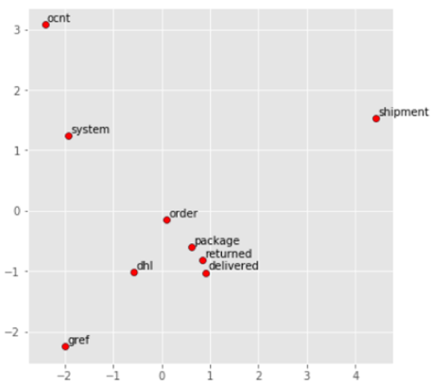
\includegraphics[scale=0.9]{content/pics/Picture_11.png}
\caption{Darstellung verschiedener Wörter in 2 Dimensionen , eigene Erstellung (Systemnamen wurden geschwärzt).}
\label{Abbildung:wordvecintuition}
\end{figure}

Abbildung \ref{Abbildung:wordvecintuition} basiert auf einem eigenen Experiment, in dem die verfügbaren Kunden-Dokumente in Kleinschreibung (etwa 330 000 Wörter; entspricht einer Größe von 2.1 Megabyte) für das Training eines eigenen Wort-Vektor-Modells verwendet wurden. Das so erzeugte Modell hat zwar spezielle Begriffe (etwa die Namen von einzelnen Projekten) aus den Dokumenten gelernt, es hat aber z. B. keine Idee davon, wie beliebige Begriffe wie ``London`` oder ``Paris`` einzuordnen sind. Diese Begriffe sind nicht einmal Teil des Vokabulars. Das zeigt, dass ein selbst trainiertes Modell nur bedingt für den Vergleich von Dokumenten geeignet ist. Es kann geschlussfolgert werden, dass das Training eines geeigneten Modells domänenspezifische Dokumente und zusätzlich einen ``allgemeinen`` Textkorpus voraussetzen würde, damit sinnvoll mit dem Modell gearbeitet werden könnte. Perspektivisch könnte also ein solches fortgeschrittenes Modell trainiert werden. 

\subsection{Ansatz 1: Ähnlichkeitsvergleich mit einem Word2Vec-Modell}

Im nachfolgenden, einleitenden Beispiel wurde die Ähnlichkeit zwischen ganzen Dokumenten berechnet. 
Aufgrund der beschriebenen Schwierigkeiten mit einem selbst trainierten Modell wird hier für die Evaluation das vortrainierte, gebrauchsfertige Wort-Vektor-Modell von spaCy verwendet. Es wurde das größte verfügbare Modell \(en\_core\_web\_lg\) gewählt. Das Modell deckt von den Begriffen aus den Kundendokumenten lediglich 91,9 Prozent der Begriffe durch Vektoren ab. Das heißt, es gibt für 8,1 Prozent der Begriffe in den Kundendokumenten keine Vektoren in dem gebrauchsfertigen spaCy-Modell\footnote{Berechnung: Wörter die keinen spaCy-Vektoren besitzen/ Gesamtanzahl der Wörter aus den Dokumenten}. Aus diesem Grund steht bereits an dieser Stelle fest, dass ein gebrauchsfertiges Modell für die Berechnung von Ähnlichkeiten recht viele wichtige Begriffe nicht berücksichtigen kann. Abbildung \ref{Abbildung:listing_1} zeigt exemplarisch, wie die Ähnlichkeit von Texten in Python auf Basis von Wort-Vektoren ermittelt werden kann. Das dargestellte Skript liefert ein Ähnlichkeitsmaß von 0.98. Es handelt sich in dem Beispiel um Dokumente, die unterschiedliche Versionen der gleichen Software beschrieben. Der gleiche Test mit doc1 aus der Abbildung und einem Dokument aus einem anderen Projekt lieferte eine Punktzahl von 0.951064. Grundsätzlich sind die Ausgaben also interpretier- und nachvollziehbar. Für das APM heißt das, dass durchaus sprachlich verwandte Dokumente und damit potenziell ähnliche Anwendungen identifziert werden können, wie im Folgenden noch weiter gezeigt wird. Zu beachten bei den Ergebnissen oben ist stets, dass einige domänenspezifische Wörter bei diesem verwendeten Modell keine Vektoren besitzen und deshalb gar nicht berücksichtigt werden können, wie bereits angedeutet. Eine Option zur Lösung des Problems bestünde darin, Vektoren komplett neu zu trainieren. 

\begin{figure}[h]
\centering
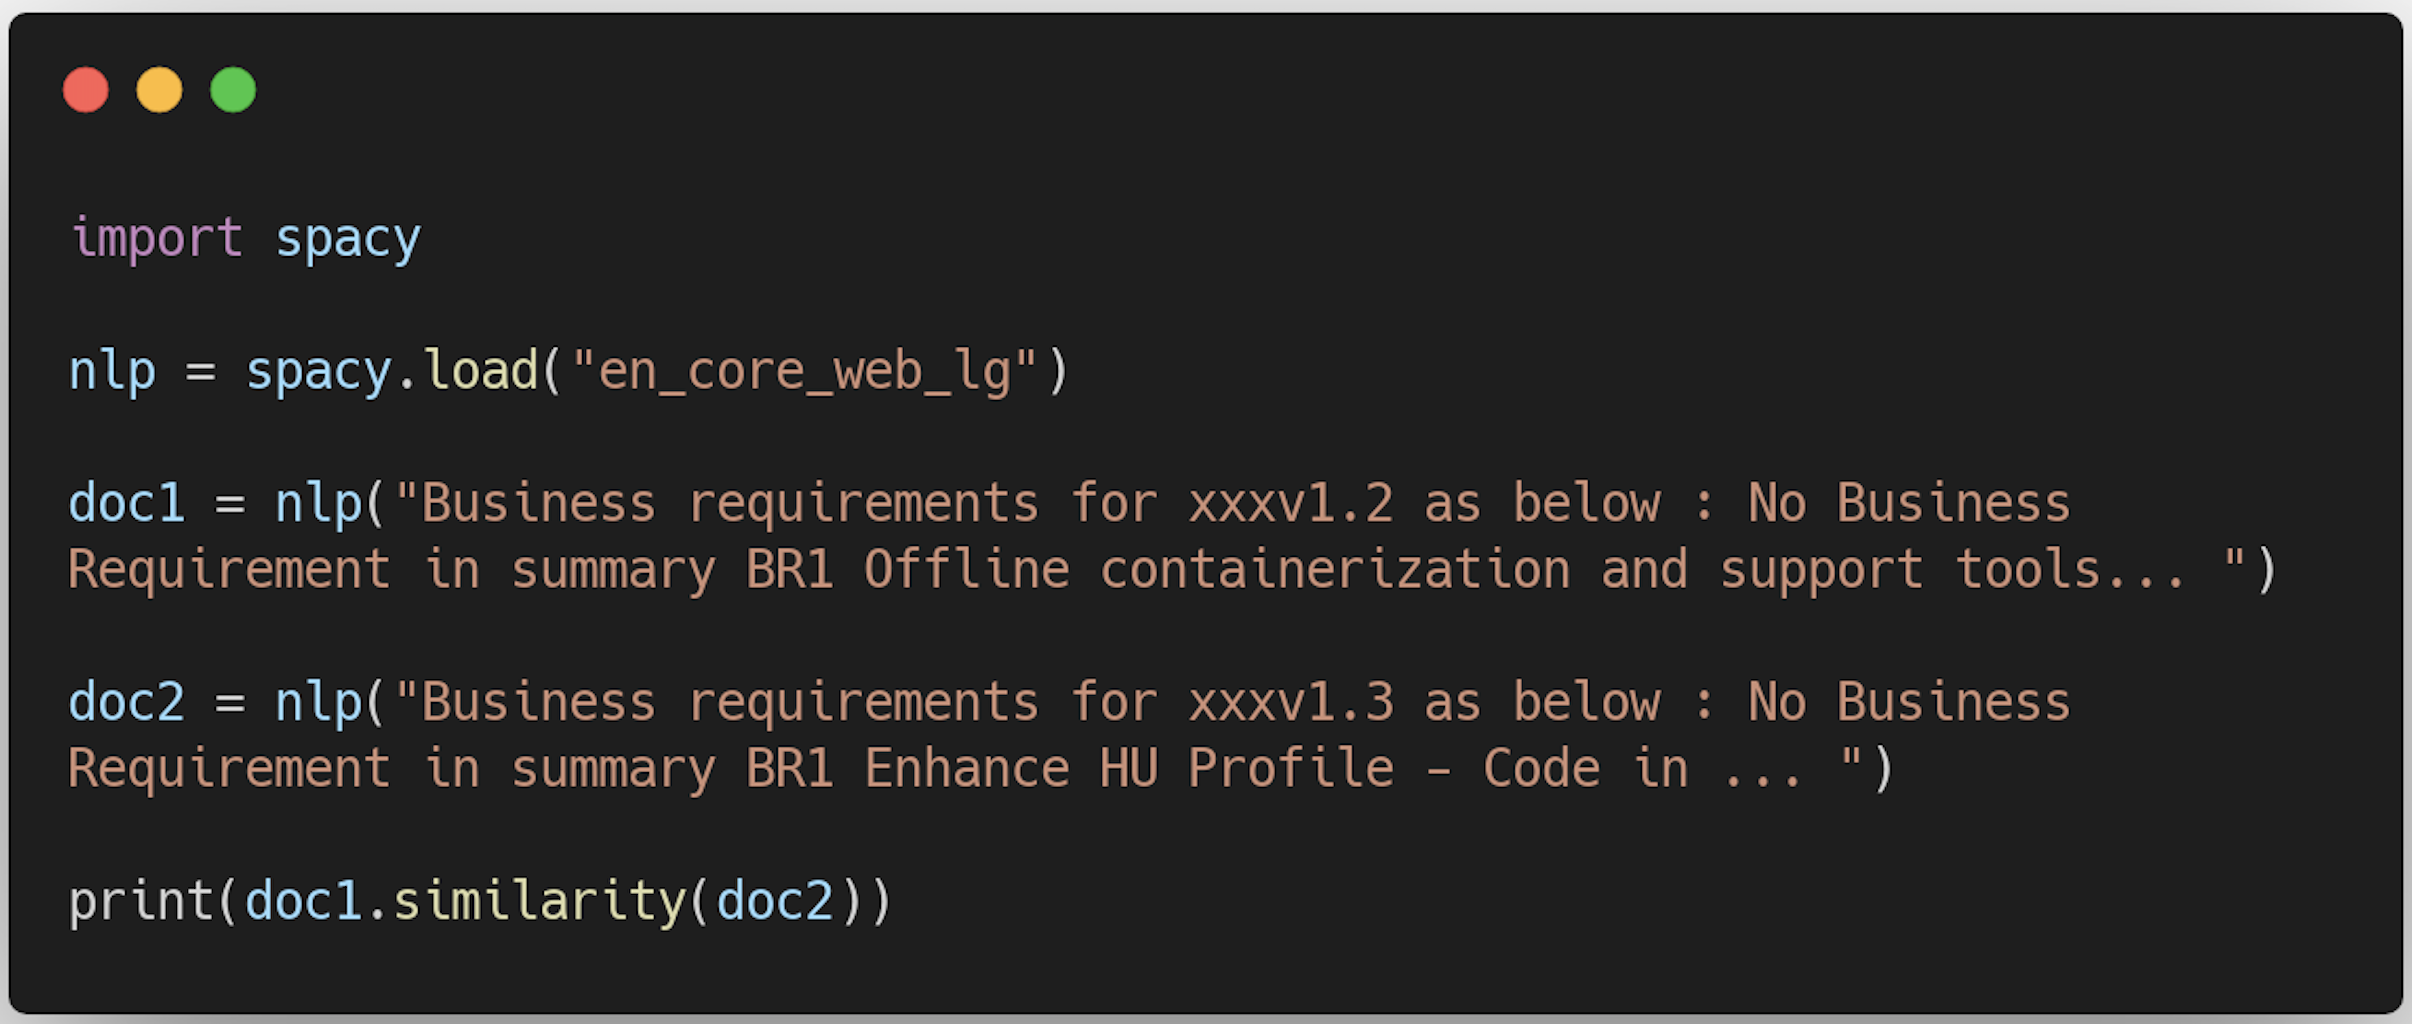
\includegraphics[scale=0.35]{content/pics/Listing_1_.png}
\caption{Similarity Berechnung mit spaCy. Die Texte wurden gekürzt.}
\label{Abbildung:listing_1}
\end{figure}

{\bf Kriterium 1: Einsetzbarkeit des Ansatzes unter den gegebenen Rahmenbedingungen}

Unten dargestellt (Abbildung \ref{Abbildung:heatmap1}) ist eine Heatmap, welche die Ähnlichkeit von Dokumenten zueinander visualisiert. Aus Datenschutzgründen werden hier nicht die Namen der Dokumente, sondern interne IDs präsentiert. In diesem Versuch wurden keine Stoppworte entfernt. Das erklärt, weshalb die Skala lediglich von 1 (zu interpretieren als ``Dokumente sind vollständig identisch``) bis 0,95 (zu interpretieren als ``Dokumente sind sich sehr ähnlich``) verläuft. In Abbildung \ref{Abbildung:heatmap2} ist das Ergebnis beim gleichen Vorgehen mit Stoppwortentfernung dargestellt. Die Skala verändert sich, d. h. Dokumente sind sich weniger ähnlich als vorher. Insgesamt sind aber kaum Unterschiede zu oben (Abbildung \ref{Abbildung:heatmap1}) erkennbar. 
 
\begin{figure}[h]
\centering
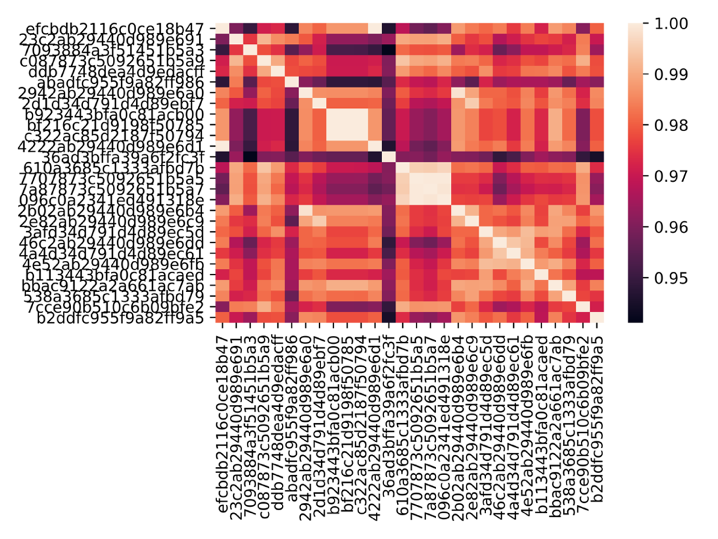
\includegraphics[scale=0.95]{content/pics/Picture_12.png}
\caption{Heatmap zur Dokumentenähnlichkeit, eigene Erstellung}
\label{Abbildung:heatmap1}
\end{figure}

\begin{figure}[h]
\centering
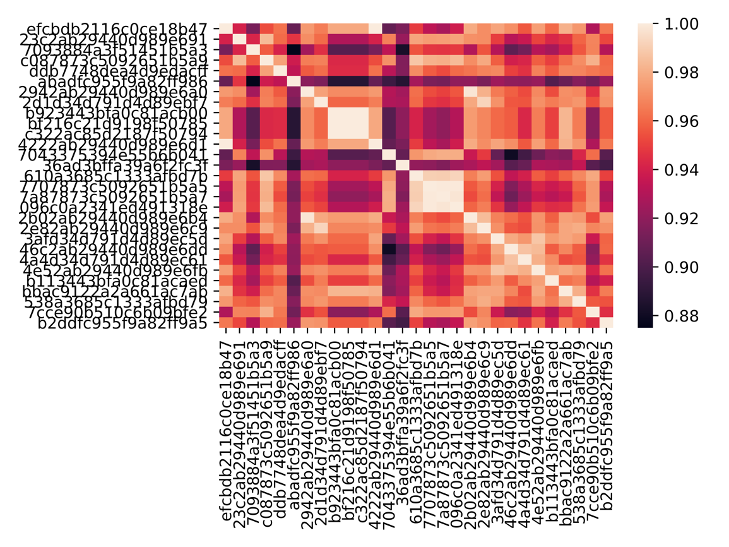
\includegraphics[scale=0.95]{content/pics/Picture_13.png}
\caption{Heatmap zur Dokumentenähnlichkeit, mit Stoppwortentfernung, eigene Erstellung}
\label{Abbildung:heatmap2}
\end{figure}

Es sind weitere Verfeinerungen denkbar, wie die Entfernung aller Verben oder Adjektive, oder die manuelle Gewichtung von bestimmten Substantiven. Ein solches Vorgehen geht in Richtung regelbasierte Sprachverarbeitung und wird daher hier nicht weiterverfolgt. 

Der Ansatz ist also mit der gegebenen Datenmenge (20-40 Dokumente) sinnvoll einsetzbar, auch wenn durch ein Training eigener Vektoren noch Verbesserungen im Hinblick auf die Ergebnisse zu erwarten sind. Er liefert zumindest Hinweise darauf, in welchen Dokumenten bzw. Projekten mit ähnlicher Sprache gearbeitet wird.
Die Metrik (etwa ``Ähnlichkeit von 0,99``) kann zum Beispiel genutzt werden, um zu überprüfen, ob ein Dokument anderen existierenden Dokumenten ähnelt. Ein Entscheider könnte sich dieses ähnliche Dokument dann noch einmal genauer ansehen, um zu prüfen, ob beispielsweise Systeme mit ähnlichen Anforderungen entdeckt wurden.

{\bf Kriterium 2: Generelle Einsetzbarkeit des Ansatzes im APM-Kontext, unter der Annahme einer beliebig großen Datenmenge}

Für Kriterium 2 gilt das gleiche wie bei Kriterium 1. Eine größere Datenmenge würde das Training eines eigenen, auf den IT-Governance-Kontext zugeschnittenen Vektor-Modells ermöglichen, wodurch noch genauere Ergebnisse zu erwarten wären.

{\bf Kriterium 3: Rechenaufwand}

Das Vergleichen von nur zwei Dokumenten mit durchschnittlich 5000 Wörtern dauert auf gewöhnlicher Hardware bereits einige Sekunden. Bei 30 Dokumenten würden sich 900 durchzuführende Vergleiche ergeben (870 wenn man Dokumente nicht mit sich selbst vergleicht). 

Von der Komplexitätsklasse ist das ein quadratisches Problem: 
$\mathcal{O}(n^2)$, wenn $n$ die Anzahl der Dokumente ist. 

Es ist also mit einer gewissen Dauer zu kalkulieren, wenn die Ähnlichkeit dynamisch berechnet werden sollte. Die Ähnlichkeit von einzelnen Dokumenten zueinander wird berechnet auf Basis der Kosinus-Ähnlichkeit, wobei zunächst von allen Vektoren der jeweiligen Dokumente der Durchschnitt berechnet wird \cite{spacy3}. Die Kosinus-Ähnlichkeit ermittelt einen Wert zwischen -1 und 1 für die Ähnlichkeit von zwei Vektoren A und B \cite[S. 84]{Gupta}:	
 
 \begin{equation}
similarity = {{\bf A} \times {\bf B} \over \|{\bf A}\| \|{\bf B}\|} = \frac{ \sum_{i=1}^{n}{{\bf A}_i{\bf B}_i} }{ \sqrt{\sum_{i=1}^{n}{({\bf A}_i)^2}} \sqrt{\sum_{i=1}^{n}{({\bf B}_i)^2}} }
\end{equation}

Der Rechenaufwand zur Erzeugung der fachspezifischen Vektoren ist abhängig von der Größe des jeweiligen Trainingskorpus. 
%\\
%\\
% \\ 

{\bf Kriterium 4: Kosten}

Es sind hier keine Kosten durch Lizensierung oder manuelle Tätigkeiten erkennbar, zumindest solange, wie mit den vortrainierten Wort-Vektoren gearbeitet wird. spaCy-Modelle verwenden die MIT-Lizenz \cite{spacy-license}, welche die kostenfreie Nutzung ermöglicht \cite{MIT}. Wenn ein Textkorpus zusammengestellt werden sollte, um eigene Vektoren zu erzeugen, dann müssten entsprechende Dokumente aus unterschiedlichen Quellen gesammelt werden, was Aufwand bedeuten würde.


\subsection{Ansatz 2: Ähnlichkeitsvergleich unter Verwendung des Paragraph-Vector-Modells (Doc2Vec)}

Das Paragraph-Vector-Modell kann ebenfalls für die Ermittlung von Ähnlichkeiten von Dokumenten eingesetzt werden \cite{Dai}. Nachfolgend wird dieses Verfahren im Kontext des APM zur Ermittlung von ähnlichen Dokumenten untersucht. Die Ähnlichkeit zwischen Dokumenten kann abgesehen von einer Heatmap (wie im vorangegangenen Abschnitt) auch über Cluster in einem Streudiagramm visualisiert werden. Diese Form der Visualisierung wird hier gewählt. Dokumente die sich ähneln, würden im Streudiagramm nahe beieinander liegen, wie nachfolgend gezeigt wird. 

{\bf Kriterium 1: Einsetzbarkeit des Ansatzes unter den gegebenen Rahmenbedingungen}

Es wird hier ein eigenes Doc2Vec-Modell trainiert. Das Verfahren Doc2Vec von gensim erzeugt für jedes Dokument einen Vektor. Diese Vektoren können je nach Parameterwahl verschiedene Dimensionen haben. Um die Vektoren in einer zweidimensionalen Ebene darstellen zu können, wurde t-SNE (t-Distributed Stochastic Neighbor Embedding, nach \cite{t-SNE}) zur Dimensionsreduktion verwendet. Es wurde davon ausgegangen, dass ähnliche Dokumente auch ähnliche Vektoren haben. Dadurch sollten in Abbildung \ref{Abbildung:doc2vec1} Cluster erkennbar sein – wie nachfolgend unter Kriterium 2 beschrieben – dies ist jedoch hier zunächst nicht der Fall. Das Verfahren eignet sich also in der Variante, die hier evaluiert wurde, nicht für den Einsatz bei einer derart kleinen Datenmenge. Ein Punkt stellt ein Dokument dar, die Farbe zeigt den Dokumententyp des Dokuments. Auf eine Beschriftung der einzelnen Datenpunkte wird aus optischen Gründen sowie aus Datenschutzgründen verzichtet. Es wurde erwartet, dass Dokumente des gleichen Dokumententyps Cluster bilden würden (vgl. die Ausführungen unter Kriterium 2)

\begin{figure}[h]
\centering
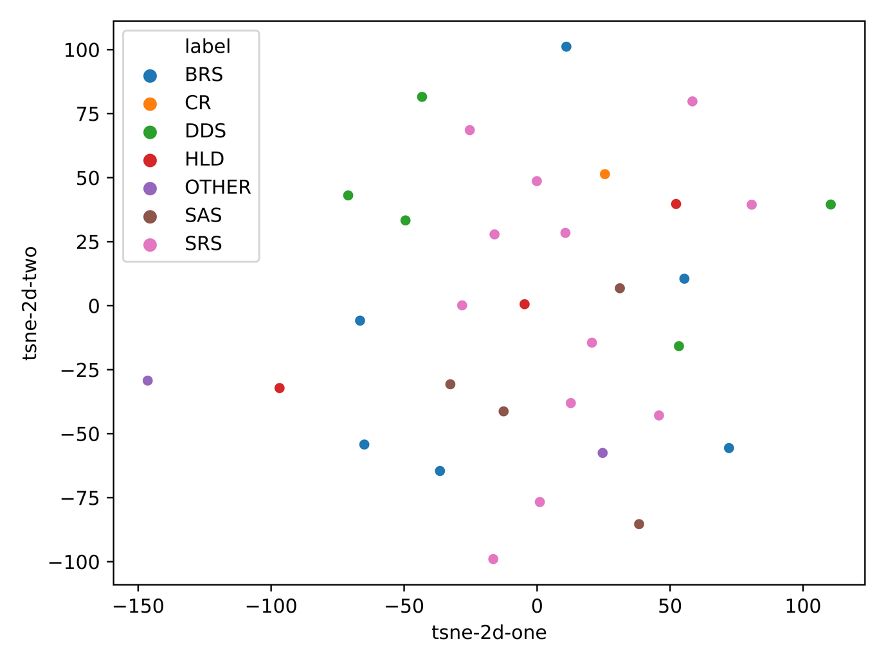
\includegraphics[scale=0.95]{content/pics/Picture_14.png}
\caption{Darstellung aller verfügbaren Dokumente, gruppiert nach Dokumententypen, eigene Erstellung}
\label{Abbildung:doc2vec1}
\end{figure}

Die Achsenbeschriftungen der Abbildung \ref{Abbildung:doc2vec1} ergeben sich lediglich durch die Dimensionsreduktion und haben keine besondere Bedeutung.

Für das APM geschlussfolgert wird, dass auch die Suche nach Dokumenten-Clustern (Anwendungs-Cluster) hilfreich sein könnte. Mit Doc2Vec und der Dimensionsreduktion kann derartiges erreicht werden, jedoch sind dazu insbesondere weitere Textdokumente notwendig.

{\bf Kriterium 2: Generelle Einsetzbarkeit des Ansatzes im APM-Kontext, unter der Annahme einer beliebig großen Datenmenge}

Man kann mit dem Verfahren grundsätzlich Cluster bilden. Dies belegt ein Beispiel aus der Literatur, auf das hier eingegangen wird. Die Dimensionsreduktion erfolgte ebenfalls mit t-SNE (vgl. Abbildung \ref{Abbildung:doc2vec2}) \cite{Dai}. 

Es werden in dem Beispiel ähnliche Wikipedia-Artikel zu Dokumenten-Clustern zusammengefasst, wodurch die generelle Einsetzbarkeit unter der Annahme einer beliebig großen Menge von Dokumenten bestätigt werden kann. Es kann allerdings nicht ausgeschlossen werden, dass die APM-Dokumente sich nicht genug voneinander unterschieden, womit das Wikipedia-Ergebnis im Kontext des APM nicht erzielt werden könnte. 

In einer realen Anwendung könnte sich z. B. durch das Auswählen einzelner Datenpunkte ein Fenster mit Details zum jeweiligen Dokument öffnen. Im Falle eines neuen Dokuments könnte die Position in der Visualisierung Hinweise darauf geben, welche ähnlichen Dokumente (bzw. Anwendungen) es bereits gibt. 

\begin{figure}[h]
\centering
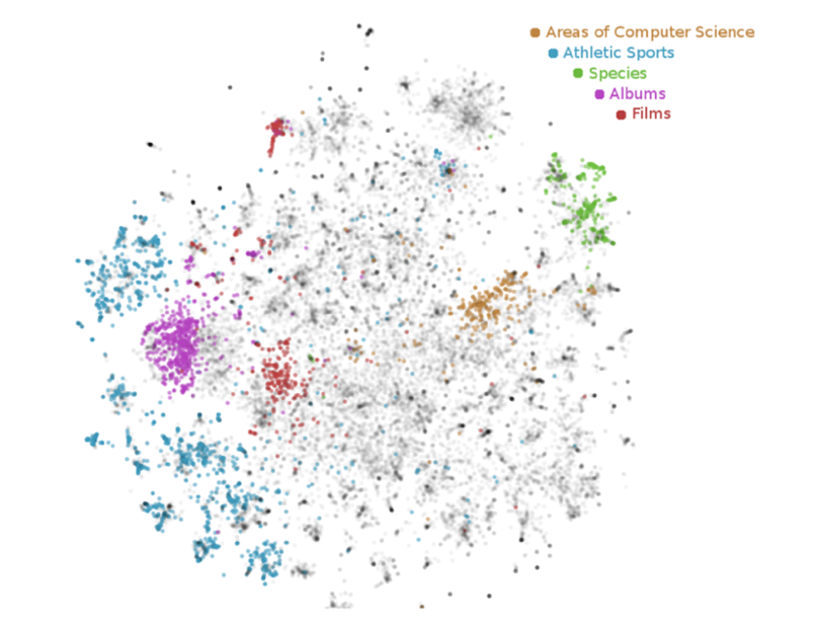
\includegraphics[scale=0.95]{content/pics/Picture_15.png}
\caption{Wikipedia-Dokumenten-Cluster, gruppiert nach Kategorien, erzeugt über Doc2Vec, aus \cite{Dai}}
\label{Abbildung:doc2vec2}
\end{figure}

%\smallskip

{\bf Kriterium 3: Rechenaufwand}

Das Erzeugen eines Scatter-Plots wie in Abbildung \ref{Abbildung:doc2vec2} erfordert zunächst das Training eines Modells. Die Trainingszeit ist abhängig von der Anzahl der Dokumente. Ein solches Modell kann auch nachts trainiert werden und dann gespeichert werden. Neue Dokumente können dann durch das Modell in Vektorform gebracht und visualisiert werden, z. B. in einer interaktiven Darstellung etwa auf einer Webseite. Die Inferenz (Erzeugung von Dokumenten-Vektoren) erfolgt ohne Verzögerungen.

{\bf Kriterium 4: Kosten}

Der Paragraph-Vector-Ansatz benötigt keine beschrifteten Beispiele und kann daher auch in Szenarien eingesetzt werden, in denen es keine beschrifteten Daten gibt \cite[S. 4]{mikolov2014}. Daher ist für das Erzeugen von Beschriftungen kein manueller Aufwand nötig, der Kosten verursachen würde. Der Ansatz benötigt dennoch aufbereitete Dokumente für das Training eines Modells. Diese sind zusammenzustellen. Lizenzkosten gibt es bei der Verwendung der Bibliothek gensim nicht \cite{gensim-license}.

\section{Ergebnisse: Bestimmung von inhaltlicher Integrität}

Bei der ``Bestimmung von inhaltlicher Integrität`` wird der Inhalt von einzelnen Kapiteln aus Anwendungsdokumentationen betrachtet. Dieser soll idealerweise das beschreiben, was erwartet wird. In einem Kapitel zu (beispielsweise) ``Anforderungen`` soll es auch um Anforderungen gehen, und nicht um etwas anderes.

\subsection{Ansatz 1: Vergleich von Durchschnitts-Wort-Vektoren}

Dieser Ansatz basiert auf durchschnittlichen Wort-Vektoren. Auf Basis einer Trainingsdatenmenge werden zunächst durchschnittliche Wort-Vektoren berechnet. Die Trainingsdatenmenge setzt sich zusammen aus mehreren Textkörpern. Die unterschiedlichen Textkörper bestehen hier aus frei zugänglichen PDF-Dokumenten aus dem Internet. Unterschieden werden dabei die folgenden Dokumententypen:

\begin{itemize}
\item Texte, in denen Anforderungen beschrieben werden (Thema Requirements)
\item Texte zu Lösungs-Architekturen (Thema Architecture bzw. Architectural Language)
\item Texte zu Software-Design (Thema Design) 
\item Texte zu Logistik-Themen (Thema Logistics)
\end{itemize}

Für jeden dieser Typen wird ein durchschnittlicher Wort-Vektor berechnet. Visualisiert wird das Vorgehen in Abbildung \ref{Abbildung:avgvec}. Nicht gezeigt wird hier der Logistik-Textkorpus.

\begin{figure}[h]
\centering
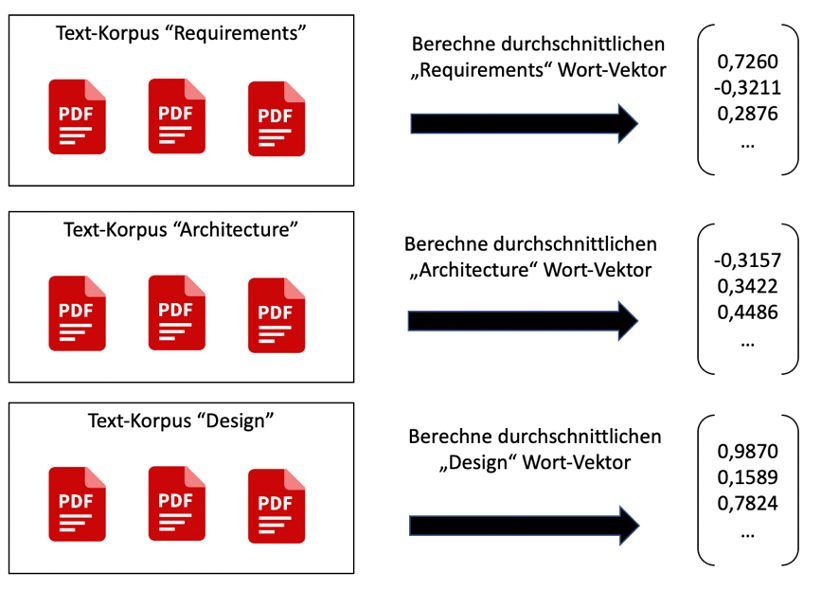
\includegraphics[scale=0.95]{content/pics/Picture_16.png}
\caption{Initiale Vorbereitung von durchschnittlichen Wort-Vektoren, eigene Erstellung}
\label{Abbildung:avgvec}
\end{figure}

Ziel ist es nun auf Kapitelebene zu schätzen, ob es in einzelnen Kapiteln von Test-Dokumenten um eines der festgelegten Themen (Requirements, Architectural Language, Design oder Logistics) geht, wie in Kapitel 3.2 beschrieben. Das Thema Logistik dient dabei als Referenz- bzw. als Vergleichskorpus. Hintergrund ist stets die Prüfung, ob ein Kapitel enthält, was es laut Vorgabe enthalten sollte. Die Zielvariable heißt ``erkanntes Thema`` – sie kann verwendet werden, um die Wahrscheinlichkeit zu messen, mit der ein Kapitel die erwarteten Inhalte enthält. Die Wahrscheinlichkeiten ergeben sich, indem für jedes Kapitel in einem zu untersuchenden Beispiel-Dokument ebenfalls Vektoren erzeugt werden. Diese werden dann mit den Durchschnitts-Vektoren verglichen (vgl. Abbildung \ref{Abbildung:avgvec2}). 

\begin{figure}[h]
\centering
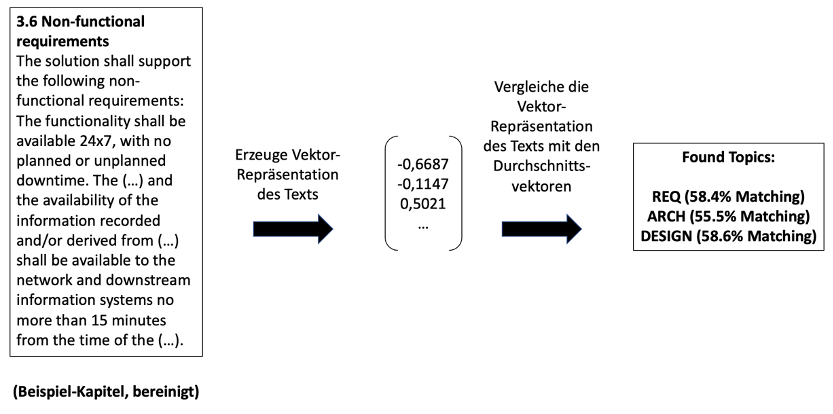
\includegraphics[scale=0.95]{content/pics/Picture_17.png}
\caption{Inferenz-Phase. Vergleich von Kapitel-Vektoren mit Durchschnitts-Vektoren, eigene Erstellung}
\label{Abbildung:avgvec2}
\end{figure}

{\bf Kriterium 1: Einsetzbarkeit des Ansatzes unter den gegebenen Rahmenbedingungen}

Als Trainingsmenge können beliebig viele Dokumente verwendet werden. Hier wurden pro Text-Korpus etwa 20 PDF-Dokumente aus dem Internet verwendet. Auf Basis dieser Dokumente wurden die Durchschnittsvektoren ermittelt. 
In Abbildung \ref{Abbildung:avgvec2} werden mögliche Resultate schon angedeutet. Die Schätzungen haben meist mit mehreren Durchschnittsvektoren Ähnlichkeiten. Daher kann hier von keiner zuverlässigen Vorhersage der Topics gesprochen werden. 
Es werden hier auch keine Metriken im Sinne einer Konfusionsmatrix präsentiert, weil Abschnitte stets mit mehreren der Topics eine Ähnlichkeit hatten. Das zeigt auch der nachfolgende direkte Vergleich von den durchschnittlichen Vektoren (vgl. Tabelle \ref{table:4}).

\begin{table}[h]
\centering
\begin{tabular}{|c|c|c|c|c|}
\hline
                      & \textbf{Logistics} & \textbf{Architecture} & \textbf{Design} & \textbf{Requirements} \\ \hline
\textbf{Logistics}    & 1                  & 0.93                  & 0.91            & 0.92                  \\ \hline
\textbf{Architecture} & 0.93               & 1                     & 0.99            & 0.98                  \\ \hline
\textbf{Design}       & 0.91               & 0.99                  & 1               & 0.99                  \\ \hline
\textbf{Requirements} & 0.92               & 0.98                  & 0.99            & 1                     \\ \hline
\end{tabular}
\caption{Vergleich der Durchschnitts-Vektoren miteinander. Der Vergleich erfolgte mit der Similarity-Funktion von spaCy.}
\label{table:4}
\end{table}

Als Ursache für die Ähnlichkeit der Vektoren (mit Ausnahme des Referenzkorpus ``Logistics``, wo durchaus eine Unterscheidung möglich ist) wird von der inhaltlichen Nähe der Text-Körper zueinander ausgegangen (vgl. etwa ``Design`` und ``Architecture``, wo eine Ähnlichkeit von 0,99 gegeben ist, die Vektoren also beinahe gleich sind. Bei Vergleichen mit ``Logistics`` ist eine derart starke Ähnlichkeit nicht gegeben). Die gewählten Topics sind sich inhaltlich sehr ähnlich, weshalb hier die sorgfältige Auswahl der Trainingsdokumente in den jeweiligen Kategorien eine Rolle spielt. Die einfache Durchschnittsbildung (averaging) führt also im Kontext des APM eher weniger zu sinnvollen Vektoren, weshalb mit einer derart geringen Datenmenge der Ansatz nicht sinnvoll genutzt werden kann.
Aus den Ergebnissen folgt jedoch, dass man mit dem Verfahren zumindest ein Gefühl dafür bekommen kann, ob die Inhalte einzelner Kapitel grob in die richtige Richtung gehen. Texte wie etwa {\textit{lorem ipsum}}, könnten als unsinnige Inhalte identifiziert werden.

{\bf Kriterium 2: Generelle Einsetzbarkeit des Ansatzes im APM-Kontext, unter der Annahme einer beliebig großen Datenmenge}

Wie oben beschrieben (vgl. Tabelle \ref{table:4}), sind die gewählten Themen, mit Ausnahme des Themas Logistics, sich inhaltlich sehr ähnlich. Das ändert sich auch bei größeren Trainingsdatenmengen nicht, da die Dokumente sich inhaltlich stets sehr ähnlich sein werden. Daher kann hier die generelle Einsetzbarkeit dieses Ansatzes nicht bestätigt werden, sofern zwischen sehr ähnlichen Themen (wie im vorliegenden Kontext) unterschieden werden soll.

Die Autoren dieser Studie \cite{dilawar} evaluierten ebenfalls verschiedene Ansätze zur Kombination von Wort-Vektoren, so wie es bis hierhin beschrieben wurde. Allerdings unterscheidet sich der Ansatz der Autoren darin, dass kein schlichter Vektor-Vergleich mit Durchschnittsvektoren durchgeführt wird. Stattdessen werden Vektor-Repräsentationen des Texts noch als Eingabe für ein Klassifizierungsverfahren verwendet, wobei ein neuronales Netz zum Einsatz kommt. Dabei handelt es sich im Prinzip um einen eigenen Ansatz. Da es in diesem Abschnitt um den Vergleich von Durchschnitts-Vektoren ging, wird der Klassifizierungsansatz hier nicht näher betrachtet, er soll aber als Möglichkeit für weitere Versuche dokumentiert werden.


{\bf Kriterium 3: Rechenaufwand}

Ein gebräuchliches Maß zur Bewertung der Ähnlichkeit ist die Kosinus-Ähnlichkeit. Der eigentliche Abgleich der Vektoren erfolgt mit dieser Metrik, unter Verwendung der spaCy-Similarity-Funktion. Details zur Kosinus-Ähnlichkeit wurden bereits in Abschnitt 4.1.1 unter Kriterium 3 beschrieben. Als Wort-Vektoren wurden hier die vortrainierten Vektoren von spaCy genutzt. Daher ist kein Aufwand für das Training notwendig, sofern das vortrainierte Modell gewählt werden soll. Alternativ können Wort-Vektoren auch selbst trainiert werden, dann wäre ein entsprechender Rechen- und Zeitaufwand zu berücksichtigen.

{\bf Kriterium 4: Kosten}

Es können frei verfügbare Software-Bibliotheken (u. a. spaCy \cite{spacy-license}, NumPy \cite{numpy-license}) verwendet werden. Kosten entstehen durch das Sammeln und das Verwalten von Dokumenten für das Training. Im vorliegenden Beispiel wurden zunächst im Internet Dokumente als Ausgangsbasis für die Durchschnittsbildung gesucht, was aufwändig wird, wenn eine hohe Anzahl an Dokumenten mit ausreichender Qualität gesucht werden soll.

\subsection{Ansatz 2: Topic Modelling mit Non-negative matrix factorization}

Wie oben bereits angedeutet, gäbe es für die Lösung des Anwendungsfalls ``Bestimmung von inhaltlicher Integrität`` weitere Möglichkeiten aus den Bereichen des überwachten, unüberwachten oder auch semi-überwachten Lernens. Mit verschiedenen Klassifizierungsverfahren können die Klassen beziehungsweise die Themen von einzelnen Kapiteln aus Text-Dokumenten geschätzt werden. In Frage kämen etwa Ansätze wie Naive Bayes, logistische Regression, neuronale Netze, und andere. Hier vorgestellt wird nun ein Ansatz auf Basis von Non-negative matrix factorization (Abk.: NMF). Zu beachten ist, dass es sich dabei nicht um ein Klassifizierungsverfahren, sondern um eine Methode aus der Kategorie des Topic Modelling handelt. Statt mit NMF könnten ähnliche Resultate auch unter Verwendung des Verfahrens Latent Dirichlet Allocation (Abk.: LDA) realisiert und evaluiert werden \cite{scikit1}.

Als Trainingskorpus wird auch hier eine Menge von Dokumenten aus dem Internet verwendet. Verwendet wurden  wiederum die Textkorpora Requirements, Architectural Language, Design sowie Logistics. Bei näherer Betrachtung des Trainingskorpus fällt auf, dass die Trainingsdokumente in den einzelnen Kategorien sich durchaus durch bestimmte, typische Begriffe auszeichnen. Diese Begriffe sind die bedeutsamsten für ein bestimmtes Thema. Zur Visualisierung dieser Begriffe von Topics können Ansätze wie NMF oder LDA genutzt werden. Diese Ansätze verwenden intern als Vorverarabeitungsschritt die TF-IDF-Metrik. Zur Schätzung des Topics eines Testdokuments kann dann das erstellte Modell genutzt werden. Zunächst folgt allerdings in Abbildung \ref{Abbildung:word-clouds} eine Visualisierung der für die Themen typischen Begriffe. Die Begriffe die von Bedeutung sind für ein Thema wurden automatisch durch das Verfahren extrahiert und sind unten dargestellt.
 
\begin{figure}[h]
\centering
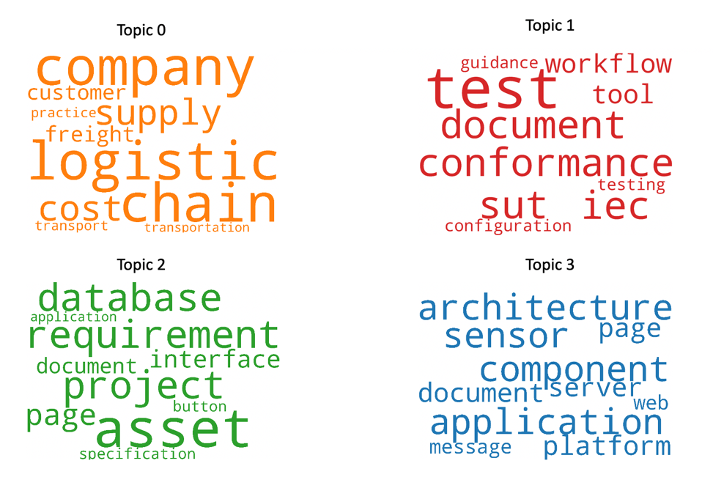
\includegraphics[scale=0.95]{content/pics/Picture_18.png}
\caption{Tag Clouds zu 4 erkannten Topics, erstellt mit NMF (eigene Erstellung)}
\label{Abbildung:word-clouds}
\end{figure}

Mit bloßem Auge erkennbar sind in Abbildung \ref{Abbildung:word-clouds} die Themen Requirements (Topic 2), Architectural Language (Topic 3) und Logistics (Topic 0). Für die Vorhersage des Topics eines neuen Dokuments (Testdokumente) werden noch weitere als die je 10 hier dargestellten Begriffe verwendet. Es handelt sich jedoch bei den Begriffen in Abbildung \ref{Abbildung:word-clouds} um jene Begriffe, die laut Modell am aussagekräftigsten für die Topics sind. Die Vorhersage des Themas eines Testdokuments liefert als Ergebnis eine Zuordnung zu einem der vier Themen. Ein Beispiel ist abgebildet in Abbildung \ref{Abbildung:nmf-inf}.

\begin{figure}[h]
\centering
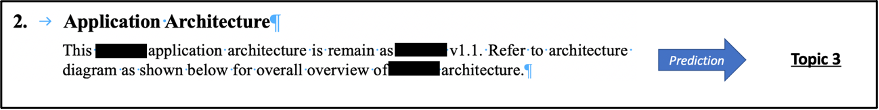
\includegraphics[scale=0.95]{content/pics/Picture_19.png}
\caption{Verwendung eines Abschnitts aus einem Testdokument für die Vorhersage des Topics, eigene Erstellung}
\label{Abbildung:nmf-inf}
\end{figure}
 
Dieses Verfahren sagt dem Nutzer lediglich, dass zum Beispiel Topic 3 als Ergebnis einer Vorhersage bestimmt wurde. Das Verfahren sagt nicht, wie das Topic zu interpretieren ist, also um welche ``Klasse`` es sich bei dem Topic handelt. Die ``Klassen`` müssen deshalb manuell auf Basis der Tag Clouds (Abbildung \ref{Abbildung:word-clouds}) bestimmt werden.

{\bf Kriterium 1: Einsetzbarkeit des Ansatzes unter den gegebenen Rahmenbedingungen}

Es wurden per Hand Text-Beispiele für Tests ausgewählt und entsprechende Beschriftungen erzeugt. Es wurden manuell 4 Texte dem Thema Software Design zugeordnet, 13 der Kategorie Requirements, und 3 wurden als Architectural Language eingeordnet. Für jedes Beispiel wird eine Schätzung mit dem NMF-Modell durchgeführt. Die Ergebnisse der Schätzungen sind unten (Tabelle \ref{tab:confusion-nmf}) dargestellt. Topic 0 (``Logistics``) kann als Kontroll-Klasse verstanden werden, die eigentlich nicht vorhergesagt werden sollte. Die Klasse ``Requirements`` könnte aus fachlicher Sicht auch in zwei Klassen functional und non-functional aufgeteilt werden. Diese Unterscheidung wurde hier nicht gemacht.

\begin{table}[h]
\centering
\begin{tabular}{|c|c|c|c|c|}
\hline
                           & \multicolumn{4}{c|}{Tatsächliche Klasse}                                  \\ \hline
\multirow{5}{*}{Schätzung} &         & Software Design & Requirements & Architectural Language \\ \cline{2-5} 
                           & Topic 0 & 0               & 0            & 0                      \\ \cline{2-5} 
                           & Topic 1 & 0               & 0            & 0                      \\ \cline{2-5} 
                           & Topic 2 & 0               & 10           & 0                      \\ \cline{2-5} 
                           & Topic 3 & 4               & 3            & 3                      \\ \hline

\end{tabular}
\caption{Konfusionsmatrix zur Darstellung der NMF-Schätzungen}
\label{tab:confusion-nmf}
\end{table}

Es wurde also für 20 Test-Abschnitte eine Vorhersage mit dem Modell erstellt werden. Das hier lediglich 20 Schätzungen erstellt wurden, liegt an den wenigen qualitativ hochwertigen Dokumenten, die für die Evaluation genutzt werden konnten. Ein Ausschnitt aus den für die Evaluation verwendeten Daten ist in Abbildung \ref{Abbildung:test-setup} abgebildet. Für die Interpretation der Konfusionsmatrix wird auf Abbildung \ref{Abbildung:word-clouds} verwiesen. Zu erkennen ist, dass etwa 77\% der Texte, die manuell als Requirements markiert wurden, auch durch das Modell in die korrekte Klasse eingeteilt wurden (10/13). Bei Architectural Language werden alle drei Beispiele in die richtige Klasse eingeteilt. Die Klasse Software Design hingegen wird in die gleiche Kategorie wie die Texte aus Architectural Language eingeteilt. Das kann daran liegen, dass sich diese beiden Kategorien inhaltlich sehr stark überschneiden. Abschnitte für ``Software Design`` stammen hauptsächlich aus DDS-Dokumenten (Detail(ed) Design Specification), Abschnitte für ``Requirements`` stammen hauptsächlich aus BRS-Dokumenten (Business Requirement Specification), Abschnitte für ``Architectural Language`` stammen hauptsächlich aus SAS-Dokumenten (Solution Architecture Statement). 

\begin{figure}[h]
\centering
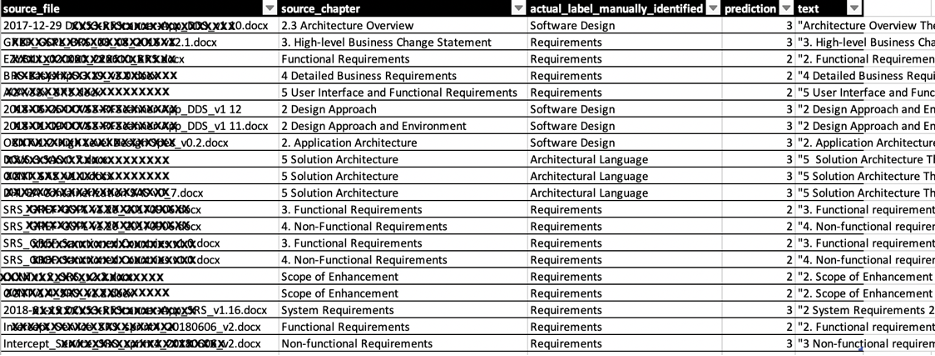
\includegraphics[scale=0.95]{content/pics/Picture_20.png}
\caption{Struktur der Daten, die für Evaluation in diesem Abschnitt genutzt wurden (geschwärzt und gekürzt)}
\label{Abbildung:test-setup}
\end{figure}

{\bf Kriterium 2: Generelle Einsetzbarkeit des Ansatzes im APM-Kontext, unter der Annahme einer beliebig großen Datenmenge}

Wie der Code im Anhang dieser Arbeit zeigt, arbeitet der Ansatz unüberwacht. Das bedeutet, dass auch größere Textmengen für die Erstellung des Modells genutzt werden könnten. Da bereits unter Kriterium 1 gezeigt wurde, dass der Ansatz durchaus Themen schätzen kann, wird das auch bei einer beliebig großen Datenmenge möglich sein. Zu beachten ist, dass die Themen sich inhaltlich stark genug voneinander unterscheiden sollten.

{\bf Kriterium 3: Rechenaufwand}

Eine Implementierung des Verfahrens ist gekapselt in der scikit-learn-Funktion NMF, weshalb auf eine detaillierte Algorithmus-Beschreibung verzichtet wird. Das Verfahren zeichnet sich jedoch durch eine polynomiale Komplexität aus. Das bedeutet, dass der Rechenaufwand je nach Parameterwahl bei der Initialisierung des Modells entsprechend stark steigen kann, je nachdem welche Parameter ausgewählt werden. Zu den Parametern zählt sowohl die Anzahl der Themen, sowie die Textmenge, die für die Modellerstellung verwendet wird \cite{scikit1}.

{\bf Kriterium 4: Kosten}

Es wurden für das Trainings des Modells aufgrund der geringen verwendbaren Datenmenge PDF-Dokumente aus dem Internet verwendet. In der Realität müsste ebenfalls eine ausreichende Trainingsdatenmenge bereitgestellt werden. Dafür sind Texte zusammenzutragen, und es ist insbesondere auf die Qualität der Texte zu achten. Dadurch entstünden Kosten. Kosten für die Nutzung des Verfahrens, z. B. unter Verwendung von Bibliotheken wie scikit-learn \cite{scikit-license}, ergeben sich zunächst nicht.

\section{Ergebnisse: Automatisierte Erzeugung von Text-Zusammenfassungen}

In Abschnitt 3.3 wird begründet, was unter den Ansätzen zur Erzeugung von Text-Zusammenfassungen verstanden wird und wofür sie sinnvoll sein können. Nachfolgend evaluiert werden zunächst ein Ansatz auf Basis von TF-IDF (Abschnitt 4.3.1), gefolgt von einem Ansatz auf Transformer-Basis (Abschnitt 4.3.2). 

\subsection{Ansatz 1: Nutzung eines extraktiven Verfahrens auf Basis von TF-IDF}

Vor der Evaluation soll kurz die Funktionsweise dieses Ansatzes skizziert werden. Die Implementierung besteht aus mehreren Schritten. Eine detaillierte Implementierung mit Kommentaren befindet sich in einem Zip-Archiv, dass dieser Arbeit beigelegt wird.

Der gesamte Textkorpus wird in einzelne Sätze aufgeteilt. Das Vorkommen von Wörtern in einzelnen Sätzen wird anschließend gezählt. Daraus kann nun die TF-Metrik berechnet werden, wie im Theorieteil beschrieben. Im Anschluss wird für jeden Begriff berechnet, in wie vielen Dokumenten dieser vorkommt.

Der nächste Schritt besteht in der Multiplikation der beiden Metriken. Sätze aus dem Text, der zusammengefasst werden soll, werden nun ausgewählt. Das geschieht, indem die TF-IDF-Werte der Begriffe innerhalb eines Satzes addiert werden. Dieser Wert wird geteilt durch die Länge des jeweiligen Satzes. Die Sätze mit den höchsten Werten gelten damit als die wichtigsten Sätze des Dokuments. Ein Grenzwert bestimmt letztendlich, welche Sätze in die finale Zusammenfassung übernommen werden.

{\bf Kriterium 1: Einsetzbarkeit des Ansatzes unter den gegebenen Rahmenbedingungen}

Es wurde für diese Evaluation eins der zur Verfügung stehenden Dokumente ausgewählt.
Um die Güte der durch den Ansatz erzeugten Zusammenfassungen objektiv bewerten zu können, werden von Menschen erzeugte Referenz-Zusammenfassungen benötigt. Diese haben in etwa die gleiche Länge wie die Zusammenfassungen, die automatisch generiert wurden. Bei der Erstellung dieser Referenz-Zusammenfassungen wurde darauf geachtet, dass möglichst viele Sätze so wie sie waren übernommen wurden, ohne manuelles Umschreiben. Es stellte sich heraus, dass die Auswahl von aussagekräftigen Sätzen auch für Menschen, die wenige Hintergrundinformationen zu den eigentlichen Inhalten der Dokumente besitzen, bereits eine Herausforderung ist.
 
Eine ideale durch ein Modell erzeugte Zusammenfassung hätte einen F-Score von 1. In diesem Fall entspräche die Zusammenfassung der durch Menschen erzeugten Referenz-Zusammenfassung. Der F-Score kann interpretiert werden als gewichteter Mittelwert von Precision und Recall \cite{scikit2}. Abbildung \ref{Abbildung:rouge-metrics} stellt sehr geringe F-Scores dar. Das zeigt, dass die automatisch generierten Zusammenfassungen recht weit entfernt von Referenz-Zusammenfassungen liegen. Die Entwicklung der Metrik hängt auch mit der Länge von erzeugten Zusammenfassungen zusammen. Die Länge wird stets kleiner bzw. sie geht gegen Null, wenn der verwendete Korpus vergrößert wird.
Referenz-Zusammenfassungen sind von Menschen mit entsprechender Sorgfalt erstellt worden. Diese Sorgfalt kann dem extraktiven Ansatz nicht bescheinigt werden, d. h. die Qualität der extraktiven Zusammenfassungen ist gering.

\begin{figure}[h]
\centering
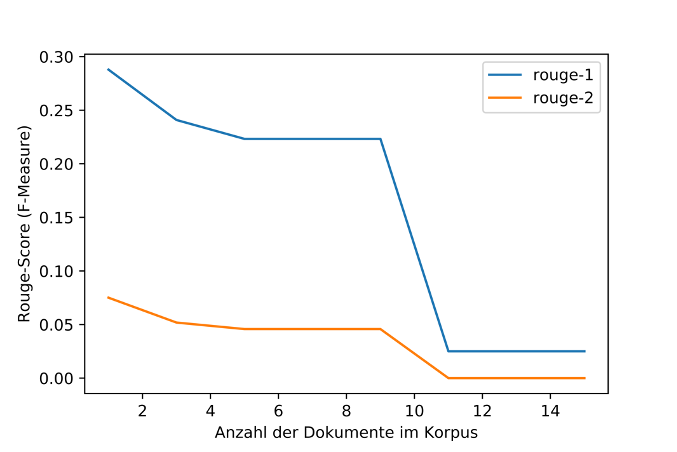
\includegraphics[scale=0.95]{content/pics/Picture_21.png}
\caption{Evaluation der Güte von Zusammenfassungen, unter Veränderung des Ausgangs-Text-Korpus. Eigene Erstellung}
\label{Abbildung:rouge-metrics}
\end{figure}

{\bf Kriterium 2: Generelle Einsetzbarkeit des Ansatzes im APM-Kontext, unter der Annahme einer beliebig großen Datenmenge}

Erwartet wurde zu Beginn, dass bei steigender Datenmenge eine Verbesserung der Rouge-Metrik erreicht werden kann. Wie in Abbildung 21 gezeigt wurde, ist eine solche Tendenz nicht erkennbar.
Eine solche Entwicklung konnte nicht beobachtet werden, weshalb das Verfahren auch bei größeren Datenmengen keine besseren Ergebnisse erbringen wird. 
Wie gezeigt wurde, wird die Güte der Zusammenfassungen von der Größe des Korpus beeinflusst. Die maximale Güte ergibt sich jedoch unter Verwendung von nur einem Text-Dokument als Korpus.

{\bf Kriterium 3: Rechenaufwand}

Dieses Verfahren verwendet eine statistische Herangehensweise und benötigt keine Iterationen oder Ähnliches für die Berechnung der Metriken, die letztendlich bestimmen, welche Sätze in die finale Zusammenfassung aufgenommen werden. Daher kann der notwendige Rechenaufwand vernachlässigt werden, wenn der Textkorpus ausreichend klein gehalten wird.

{\bf Kriterium 4: Kosten}
Wenn davon ausgegangen wird, dass die durch das Verfahren erzeugten Zusammenfassungen sinnvoll genutzt werde könnten, dann würde das Verfahren keine Kosten verursachen, da keine Beschriftungen zu erzeugen sind und Lizenzkosten nicht zu erwarten sind.

\subsection{Ansatz 2: Nutzung eines abstraktiven Verfahrens auf Transformer-Basis}

Im Vergleich zu den extraktiven Verfahren ist das Gebiet der abstraktiven Verfahren zur Erzeugung von Text-Zusammenfassungen eher Gegenstand aktueller Forschung, als eine Klasse von in der Praxis nutzbaren Verfahren \cite[S. 261]{Gupta}. Abbildung \ref{Abbildung:t5} zeigt die erzielten Ergebnisse in einem eigenen Versuch. Evaluiert wird hier das von Google-Forschern entwickelte Modell T5: Text-To-Text-Transfer-Transformer \cite{Raffel}.

\begin{figure}[h]
\centering
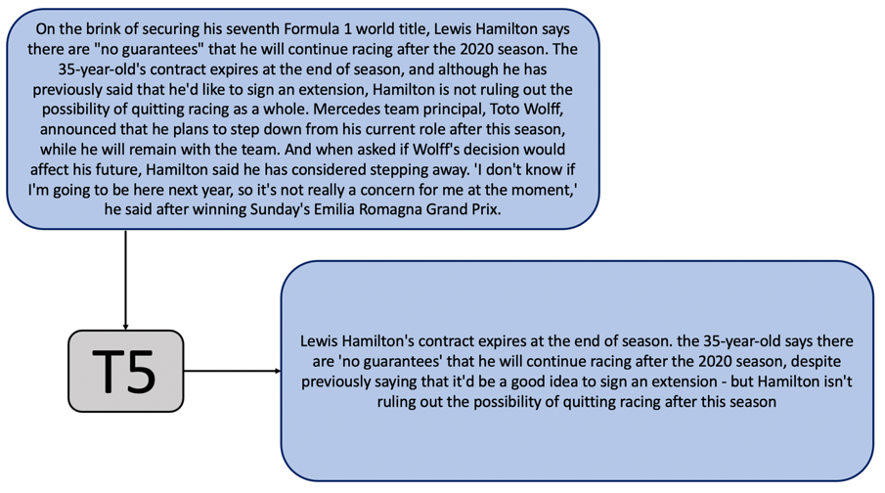
\includegraphics[scale=0.95]{content/pics/Picture_22.png}
\caption{Veranschaulichung eines abstraktiven Verfahrens. Eigene Erstellung in Anlehnung an \cite{Raffel}}
\label{Abbildung:t5}
\end{figure}

{\bf Kriterium 1: Einsetzbarkeit des Ansatzes unter den gegebenen Rahmenbedingungen}

Es ist möglich, ein vorbereitetes Modell  zu verwenden. Auf dieser Grundlage kann eine Fein-Abstimmung durchgeführt werden. Damit könnte erreicht werden, dass das Modell speziell auf Governance-Themen abgestimmt wird. Die Implementierung der Methode wurde im Rahmen der vorliegenden Evaluation in Python realisert. Dafür konnte das Package Transformers (v3.0.2) verwendet werden. Es ermöglicht die Verwendung von vortrainierten Modellen unter dem Slogan ``state-of-the-art NLP for everyone`` \cite{Transformers}.

Es wurden in einer Veröffentlichung CNN/ Daily Mail-Nachrichtentexte unter Verwendung des Modells zusammengefasst und diese Zusammenfassungen wurden mit der Rouge-Metrik evaluiert. Die Ergebnisse dieses Ansatzes setzen neue Maßstäbe bei der Qualität von automatisch generierten Zusammenfassungen \cite[S. 39]{Raffel}. Daher kann gesagt werden, dass die Qualität der Zusammenfassungen als gut eingestuft werden kann, sofern eine Fein-Abstimmung auf den jeweiligen Kontext stattgefunden hat. Die maximale Länge der Eingabe-Sequenz des T5-Modells beträgt nach aktuellem Stand 512 Tokens. Damit können als Eingabe für Zusammenfassungen bislang nur Texte mit maximal 512 Wörtern verwendet werden \cite[S. 39]{Raffel}. Das reicht maximal zur Erzeugung der Zusammenfassung einzelner Abschnitte, die dann kombiniert werden könnten. Das würde jedoch nicht dazu beitragen, dass die wichtigsten Informationen aus einem Text extrahiert werden, was hier eigentlich angestrebt werden sollte.

Longformer (The Long-Document Transformer) ist ein Transformer-Ansatz, der als Alternative zum T5-Modell in Frage käme. Hier wird kontinuierlich versucht die maximale Sequenzlänge der Eingabe zu erhöhen, dennoch gibt es auch hier derzeit noch Beschränkungen auf 4096 Tokens als Eingabe-Sequenz \cite{Longformer} \cite{Longformer2}, was ebenfalls als nicht ausreichend beurteilt werden muss.

Als Fazit wird festgehalten, dass sich die Ansätze noch zu sehr im Entwicklungsstadium befinden und durch die Beschränkung auf sehr kleine Eingabesequenzen keine sinnvollen Ergebnisse im vorliegenden Kontext erzielt werden können. Die notwendige Datenmenge für eine Feinabstimmung wird nachfolgend erläutert. Vorweggenommen werden soll, dass 20-40 Textdokumente dafür nicht ausreichend sind. Unter den gegebenen Rahmenbedingungen ist dieses abstraktive Verfahren also nicht sinnvoll einsetzbar.

{\bf Kriterium 2: Generelle Einsetzbarkeit des Ansatzes im APM-Kontext, unter der Annahme einer beliebig großen Datenmenge}

Wie in Abbildung \ref{Abbildung:t5} verdeutlicht wird, sind grundsätzlich Zusammenfassungen generierbar. Auch im Kontext der IT-Governance geht das, wobei das oben dargestellte Beispiel nur zur Verdeutlichung des Ansatzes dient. Bei der Erstellung des vortrainierten Modells wurde mit dem Colossal Clean Crawled Corpus (C4) eine Datenmenge verwendet, die aus hunderten Gigabytes bereinigten Text aus dem Internet besteht \cite[S. 5-7]{Raffel}. Bei Texten aus dem Internet ist davon auszugehen, dass diese anders zusammengesetzt sind als die Software- oder Architektur-Dokumentationen, um die es im vorliegenden Kontext geht. Daher ist ein solches vortrainiertes Modell noch nicht abgestimmt für den Anwendungsfall. Es sind für eine Fein-Abstimmung entsprechend viele Trainingsdaten notwendig. In einer Veröffentlichung wurde die Fein-Abstimmung auf Basis des CNN-Daily Mail-Datensatzes durchgeführt \cite[S. 37]{Raffel}. Die Größe dieses Datensatzes liegt bei 1.27 Gigabytes. Mit einer solchen Größe ließen sich, wie unter Kriterium 1 bereits beschrieben wurde, auch im APM-Kontext hochwertige Zusammenfassungen erzeugen, allerdings mit der Beschränkung auf 512 Tokens als Eingabesequenz.

Die Fein-Abstimmung ist insbesondere von Bedeutung, weil IT-Dokumentationen in unterschiedlichen Regionen der Welt geschrieben worden sein können. Grammatikalische Regeln werden daher nicht immer eingehalten und Formulierungen können durch lokale Besonderheiten geprägt sein. Vortrainierte Sprachmodelle allein sind daher weniger geeignet, um sinnvolle Zusammenfassungen aus den Dokumentationen zu erzeugen. Ein weiteres Hindernis stellen Abbildungen dar, auf die in den Text-Dokumenten nicht ausreichend eingegangen wird – sie enthalten häufig wichtige Informationen, die durch NLP-Verfahren alleine nicht berücksichtigt werden können. Es müssten zusätzlich weitere ML-Ansätze zur Bildverarbeitung angewendet werden, um optimale Ergebnisse erzielen zu können. Zusammengefasst könnte mit entsprechendem Aufwand eine Feinabstimmung erreicht werden, aufgrund der Beschränkung auf 512 Tokens ist der Ansatz der hier untersucht wurde jedoch (noch) nicht für das APM geeignet.

{\bf Kriterium 3: Rechenaufwand}

Die Zusammenfassungs-Funktionalitäten können unter Verwendung der Bibliotheken direkt genutzt werden, dann allerdings zunächst ohne Fein-Abstimmung. Diese Inferenz dauert auf gängiger Hardware wenige Sekunden, wie beispielhafter Code zeigt, der im Anhang der Arbeit zu finden ist. Versuche der T5-Autoren deuten darauf hin, dass mit mindestens einigen Stunden für die Feinabstimmung zu rechnen ist \cite{Raffel}.

{\bf Kriterium 4: Kosten}

Die Modelle (z. B. t5-small \cite{t5}) sowie die Transformer-Bibliothek \cite{Transformers} sind frei verfügbar. Die vortrainierten Modelle stehen zur Verfügung und können verwendet werden. Nicht zu vernachlässigende Kosten können entstehen durch die Zusammenstellung von Trainingsdaten für die Feinabstimmung eines Modells. Das bedeutet, dass für die Feinabstimmung von Menschen erstellte Zusammenfassungen benötigt werden. Wie beschrieben wurde, kann sich am CNN/ Daily Mail-Beispiel orientiert werden, wo mehrere Gigabytes an Text (Original-Texte + Zusammenfassungen) verwendet wurden. 

\section{Ergebnisse: Automatisierte Schnittstellen-Erkennung}

Die beiden nachfolgenden Ansätze verwenden beschriftete Beispiele für das Training eines Klassifikationsmodells. Die so trainierten Modelle können anschließend genutzt werden, um einzelne Sätze von Textdokumenten in eine der beiden Klassen ``Technisches Interface (TI)`` oder ``kein technisches Interface`` einzuordnen. Wenn die Vorhersage des Modells einem Satz aus der Testmenge die Klasse TI zuteilt, dann kann diese Vorhersage genutzt werden, um Sätze zu identifizieren, in denen eine technische Schnittstelle beschrieben wird. Die Genauigkeit (accuracy) dieser Vorhersage gilt es zu maximieren. Die Qualität und die Menge der Trainingsdaten haben entscheidenden Einfluss auf die Qualität der Vorhersage, wie nachfolgend beschrieben werden soll.

\subsection{Ansatz 1: Klassifizierung auf Grundlage eines BERT-Modells}

BERT, ein vortrainiertes Transformer-Modell, wird hier für die Klassifizierung verwendet, indem das vortrainierte Modell per Fine-Tuning auf den vorliegenden Kontext abgestimmt wird. Dabei werden weitere Schichten eines neuronalen Netzes trainiert, die hinter denen das BERT-Modells liegen, um eine Klassifizierungsaufgabe lösen zu können, wie beschrieben z. B. in \cite[S. 2]{Tang}. Dieser Ansatz heißt Transfer-Learning. Das BERT-Modell kennt bereits grundlegende Eigenschaften von natürlicher Sprache. Es wurde trainiert unter Verwendung des BookCorpus mit 800 Millionen Wörtern sowie der gesamten Englischsprachigen Wikipedia (2500 Millionen Wörter) \cite{devlin}.

{\bf Kriterium 1: Einsetzbarkeit des Ansatzes unter den gegebenen Rahmenbedingungen}

Die für die Feinabstimmung verwendeten Daten setzen sich zusammen aus 195 positiven Beispielen (Klasse TI), und 195 negativen Beispielen (zur Hälfte Sätze zu User Interfaces, zur anderen Hälfte Sätze vollständig ohne Interface-Information). Sie wurden manuell beschriftet. Es werden 70\% der Daten für das Training verwendet, 15\% für das Testen, und 15\% für die Validierung. Die Sätze wurden in einem vorausgegangenen Arbeitsschritt mit einem Ansatz, der auf Ontologien basiert, aus den Textdokumenten des Kunden extrahiert. Der erste Versuch ergab einen f1-score von 70\% (vgl. Abbildung \ref{Abbildung:bert-confusion}). Die interessierende Klasse TI ist erkennbar über die Ausprägung 1. Die Ausprägung 0 gibt an, dass die Vorhersage ``kein TI`` lautete. Die 70\% sind zunächst ein Zeichen dafür, dass Overfitting hier nicht unbedingt ein Problem darstellt. Bei einer verdächtig hohen Genauigkeit müsste davon ausgegangen werden.
 
\begin{figure}[h]
\centering
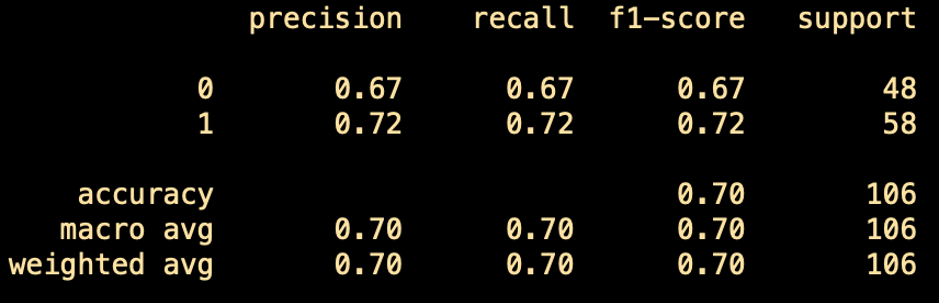
\includegraphics[scale=0.95]{content/pics/Picture_23.png}
\caption{Klassifizierungsergebnisse unter Verwendung von BERT nach der Feinabstimmung. Eigene Bildschirmaufnahme}
\label{Abbildung:bert-confusion}
\end{figure}

Die praktische Einsetzbarkeit in einem realen Szenario bei einer Erkennungsgenauigkeit von (etwa) zwei aus drei Fällen ist fraglich. Angemerkt werden muss, dass sowohl Trainings- als auch Testsätze aus dem gleichen Textkorpus stammen. Zur Folge hätte dies, dass in Produktion, d. h. bei Verwendung eines komplett anderen Dokuments, geschrieben in anderer Art- und Weise, das Modell viel schlechtere Leistung erbringen könnte, als bei den hier vorgestellten Ergebnissen vermutet werden kann. Nachfolgend soll diese Vermutung anhand eines Beispiels evaluiert werden. Es wird eine ``Requirement Specification`` aus dem Internet verwendet, um darin vorkommende Sätze in eine der beiden Klassen (``TI`` oder ``kein TI``) einzuteilen. Interessant ist, dass dieses Verfahren zunächst nicht direkt eine Klasse als Vorhersage ausgibt, sondern zwei Werte. Das sind die direkten Ausgaben des neuronalen Netzes, das für die Klassifizierung verwendet wird. Es wird der absolut größere Wert verwendet für die Bestimmung der Klasse. Eindeutig als ``kein technisches Interface`` (Klasse 0) können damit Sätze bestimmt werden, die offensichtlich kein Interface beschreiben (Abbildung \ref{Abbildung:bert-0}). Bei längeren Sätzen sind in diesem Beispiel allerdings auch viele Sätze dabei, die nichts mit Interfaces zu tun haben, aber als solche klassifiziert wurden (Abbildung \ref{Abbildung:bert-1}).

\begin{figure}[h]
\centering
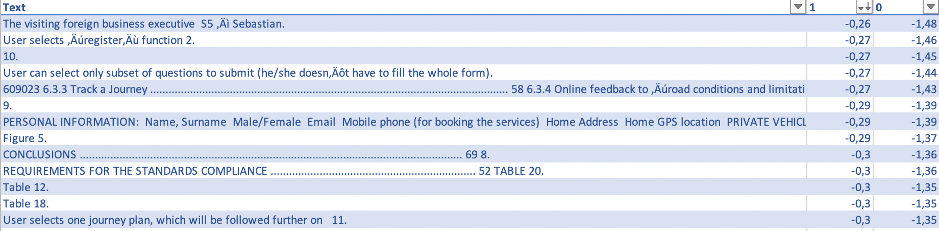
\includegraphics[scale=0.95]{content/pics/Picture_25.png}
\caption{Klasse 0 (``kein TI``) gewinnt und bestimmt damit die Vorhersage. Eigene Bildschirmaufnahme}
\label{Abbildung:bert-0}
\end{figure}

\begin{figure}[h]
\centering
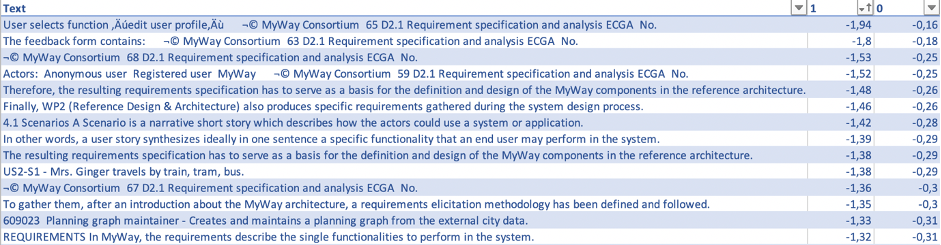
\includegraphics[scale=0.95]{content/pics/Picture_26.png}
\caption{Beispiele, bei denen Klasse 1 als Vorhersage bestimmt wurde. Eigene Bildschirmaufnahme}
\label{Abbildung:bert-1}
\end{figure}

Es wird festgehalten, dass die Feinabstimmung mit der gegebenen Datenmenge nicht ausreichend ist, um in der Praxis mit dem Ansatz sinnvolle Ergebnisse zu erreichen. Die Kernaussage ist aber, dass der Ansatz im Sinne eines Proof-of-Concepts funktionsfähig und in der Perspektive vielversprechend ist.

{\bf Kriterium 2: Generelle Einsetzbarkeit des Ansatzes im APM-Kontext, unter der Annahme einer beliebig großen Datenmenge}

Um die Güte des Verfahrens messen zu können, wären weitere beschriftete Daten notwendig. Diese müssen in ausreichender Qualität vorhanden sein, und am besten durch Experten beschriftet worden sein. Es wäre auch denkbar, dass mehrere Experten die Beschriftungen vergeben und letztendlich nur die Beschriftung für das Training verwendet wird, die von mehreren Personen als Beschriftung ausgewählt wurde. Damit würden Zweifel eliminiert werden, darüber welche Klasse die richtige für einzelne Sätze ist. In anderen Veröffentlichungen wird von Genauigkeiten von bis zu 97\% bei ausreichend großen Datenmengen berichtet \cite{Tang}. Daher wird zusammengefasst, dass dieser Ansatz generell einsetzbar sein könnte, um Schnittstellen in Texten zu identifizieren, allerdings erst dann, wenn beschriftete Trainings-Beispiele in ausreichender Menge vorliegen.

{\bf Kriterium 3: Rechenaufwand}

Es wird lediglich die Fein-Abstimmung eines BERT-Modells durchgeführt. Ein großer Teil der Gewichtungen des Netzes ist also bereits verfügbar und muss nicht erneut berechnet werden \cite{bert}.
Das Training kann auf einer CPU oder auf einer GPU durchgeführt werden\footnote{vgl. Code im Anhang}. Die Dauer der Fein-Abstimmung ist stets abhängig davon welche Prozessorarchitektur verwendet werden kann. Außerdem ist sie von gewählten Hyperparametern (Epochen/ Learning Rate, etc.) abhängig. Auf einer CPU dauert die Feinabstimmung länger als auf einer GPU. Es muss mit einigen Minuten auf gewöhnlicher Hardware kalkuliert werden. Die Inferenz (Vorhersage) nach dem Training ist ohne größere Verzögerungen möglich.

{\bf Kriterium 4: Kosten}

Das Auszeichnen von Sätzen ist der Kostentreiber bei diesem Ansatz. Dieser Aufwand erfolgt bei Einführung des Ansatzes, im Laufe der Zeit können jedoch Anpassungen notwendig werden. Es wäre denkbar, dass mehrere Menschen über die Beschriftungen entscheiden, etwa nach dem Mehrheitsprinzip: es wird die Beschriftung von dem Modell verwendet, für die sich die Mehrheit entschieden hat. Da Kenntnisse auf Expertenniveau benötigt werden, kann dieser Ansatz entsprechende Kosten verursachen. Lizenzkosten sind nicht zu erwarten, da die Apache-2.0-Lizenz verwendet wird \cite{bert}.

\subsection{Ansatz 2: Klassifizierung mit logistischer Regression auf Basis von N-Grammen}

Das Ziel ist hier wie bereits schon in Abschnitt 4.4.1 die Erkennung von Interface-Sätzen. In Kontrast zu dem vorangegangenen Ansatz, der auf Deep Learning sowie dem Transformer-Modell basierte, wird hier nun ein anderer Ansatz untersucht. Dadurch können die Ergebnisse der beiden Klassifizierungs-Ansätze besser eingeschätzt und verglichen werden. 

Es handelt sich bei diesem Ansatz um die Klassifizierung von einzelnen Sätzen mit logistischer Regression. Es wird auf Wort-Vektoren oder ein vortrainiertes Transformer-Modell verzichtet und stattdessen werden aus Texten nur N-Gramme gebildet, die später als Features für die logistische Regression verwendet werden. Es werden die typischen Schritte \cite[S. 124]{Gupta} für eine Klassifizierung verfolgt. Die Implementierung ist überschaubar, weshalb sie anhand des schematischen Programmcodes (Abbildung \ref{Abbildung:lr-code}) beschrieben werden sollen. Der Code ist gekürzt, unter anderem wurden die Importe der Bibliotheken entfernt.

\begin{figure}[h]
\centering
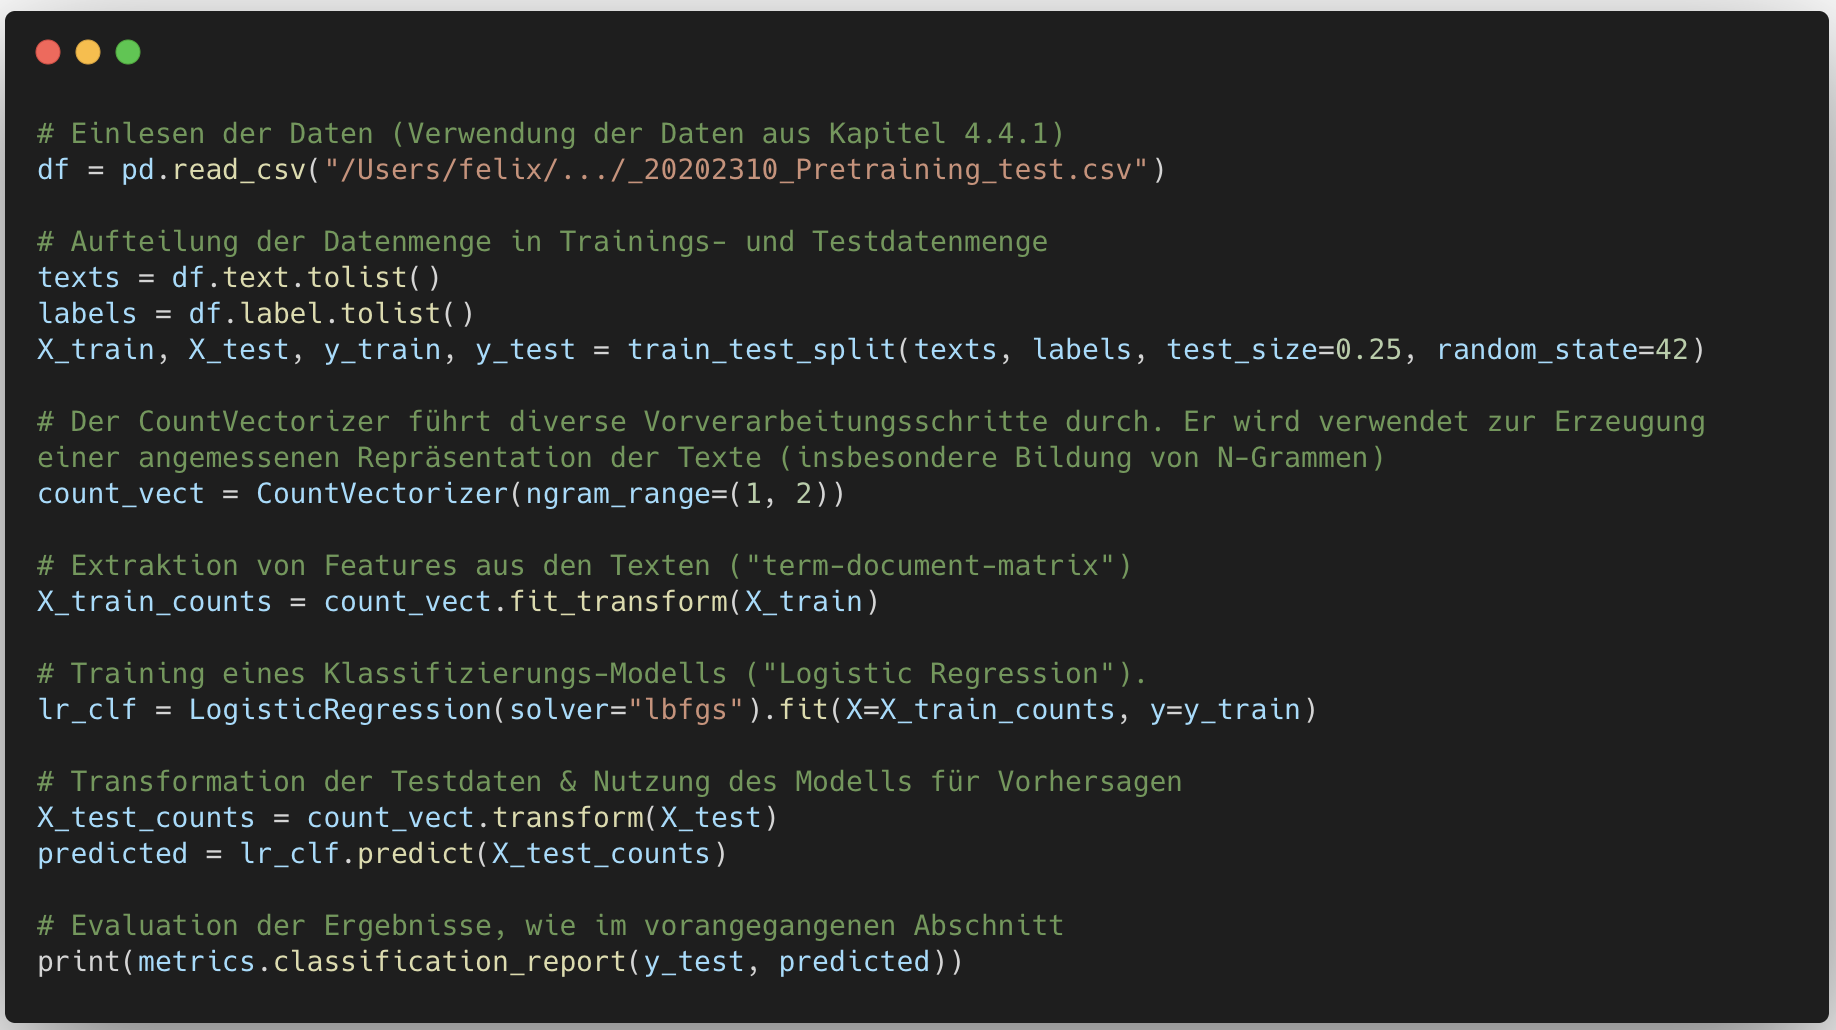
\includegraphics[scale=0.4]{content/pics/Listing_2_.png}
\caption{Klassifizierung mit logistischer Regression. Eigene Erstellung}
\label{Abbildung:lr-code}
\end{figure}

{\bf Kriterium 1: Einsetzbarkeit des Ansatzes unter den gegebenen Rahmenbedingungen}

Es werden nachfolgend in \ref{Abbildung:lr-test} die Ergebnisse des Versuchs aus \ref{Abbildung:lr-code} präsentiert.

\begin{figure}[h]
\centering
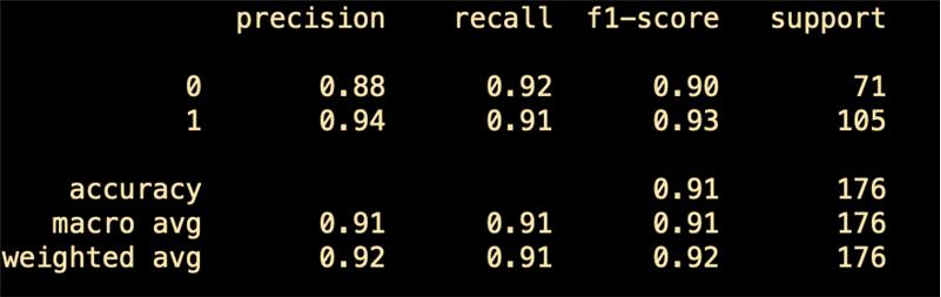
\includegraphics[scale=0.95]{content/pics/Picture_27.png}
\caption{Ergebnisse der Klassifizierung von Sätzen aus der Testmenge. Eigene Bildschirmaufnahme}
\label{Abbildung:lr-test}
\end{figure}

Diese zunächst gutaussehenden Ergebnisse können wohl durch Overfitting erklärt werden. Dieser Umstand ist der geringen Datenmenge geschuldet. Ein Versuch mit einem komplett anderen Dokument (vgl. \ref{Abbildung:lr-eval}) etwa klassifiziert 153 der insgesamt 494 Sätze aus diesem Dokument in die TI-Klasse (entspricht Klasse 1 in \ref{Abbildung:lr-eval}; es geht um das gleiche Dokument bzw. das gleiche Vorgehen wie in 4.4.1). Zu sehen ist, dass Sätze in Klasse 0 (``kein technisches Interface``) tatsächlich häufig korrekt klassifiziert wurden. Genauso häufig werden aber auch Sätze, die offensichtlich nichts mit Interfaces zu tun haben, in Klasse 1 (technisches Interface) klassifiziert, was nicht korrekt ist.

\begin{figure}[h]
\centering
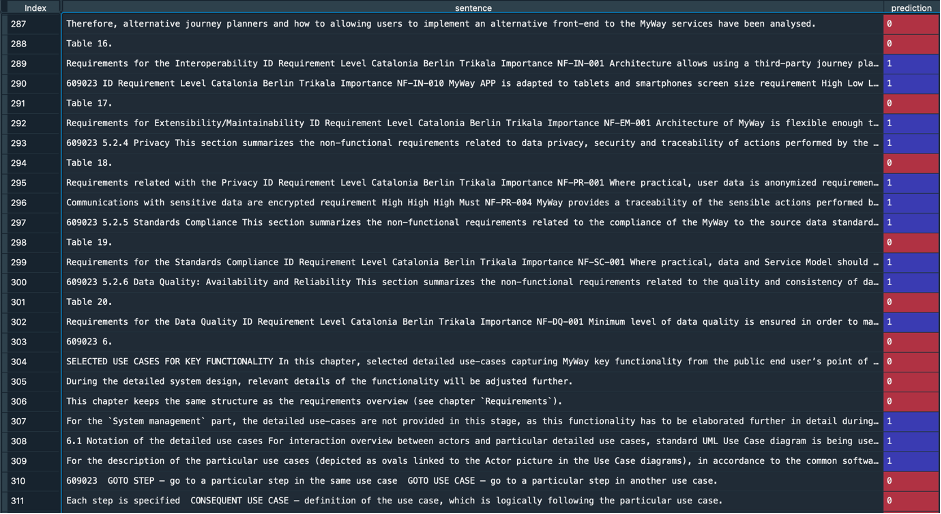
\includegraphics[scale=0.95]{content/pics/Picture_28.png}
\caption{Einige Vorhersagen für ein Evaluations-Dokument. Eigene Bildschirmaufnahme}
\label{Abbildung:lr-eval}
\end{figure}

Deshalb kann die produktive Einsetzbarkeit des Verfahrens unter den gegebenen Rahmenbedingungen mit relativ wenigen Datensätzen für das Training eines Modells nicht bestätigt werden.

{\bf Kriterium 2: Generelle Einsetzbarkeit des Ansatzes im APM-Kontext, unter der Annahme einer beliebig großen Datenmenge}

Hier \cite{Vogelsang} wurde eine ähnliche Klassifikation durchgeführt. Die Autoren verwendeten 89 Text-Dokumente für das Training des Klassifikationsmodells. Erreicht wurde, dass 4 von 5 Test-Dokumenten korrekt klassifiziert wurden – ein grundsätzlich gutes Ergebnis, erreicht mit einer kleinen Trainingsmenge. Es kann jedoch gesagt werden, dass bei steigenden Trainingsdatenmengen recht zuverlässige Ergebnisse erzielt werden können, was auch für den vorliegenden Kontext gelten würde. Damit kommt das Verfahren bei ausreichender Trainingsdatenmenge durchaus für den Einsatz in Frage. 

{\bf Kriterium 3: Rechenaufwand}

Die Vorverarbeitung, sowie das Training des Modells erfolgen in wenigen Sekunden. Die Anwendung zur Vorhersage von neuen Datensätzen erfolgt ebenfalls in wenigen Sekunden.

{\bf Kriterium 4: Kosten}

scikit-learn kann kostenfrei genutzt werden \cite{scikit-license}. Zur Verbesserung und Weiterentwicklung des Modells müssen weitere Sätze beschriftet und weitere Dokumente gesammelt werden. Das erzeugt manuellen Aufwand.

\section{Zusammenfassung der Ergebnisse}

Dieser Abschnitt stellt die Ergebnisse der Evaluation zusammenfassend in einer Übersicht dar. Des Weiteren enthält Tabelle \ref{tab:zusammenfassung} eine Handlungsempfehlung zum weiteren Vorgehen mit den Verfahren.


% Please add the following required packages to your document preamble:
% \usepackage{multirow}
\begin{table}[h]
\centering
\begin{tabular}{|c|c|c|}
\hline
\textbf{Kategorie}                                                                                                & \textbf{Ansatz}                                                                                              & \textbf{\begin{tabular}[c]{@{}c@{}}Handlungsempfehlung/ \\ Zusammenfassung\end{tabular}}                                          \\ \hline
\multirow{2}{*}{\begin{tabular}[c]{@{}c@{}}Ermittlung \\ von \\ Ähnlichkeiten\end{tabular}}                       & \begin{tabular}[c]{@{}c@{}}Mit einem (vortrainierten) \\ Word2Vec-Modell\end{tabular}                        & \begin{tabular}[c]{@{}c@{}}Gute Grundlage. \\ Weiterentwicklung \\ kann sinnvoll sein.\end{tabular}                               \\ \cline{2-3} 
                                                                                                                  & \begin{tabular}[c]{@{}c@{}}Unter Verwendung des \\ Paragraph-Vector-Modells (Doc2Vec)\end{tabular}           & \begin{tabular}[c]{@{}c@{}}Kann bei ausreichenden\\ Datenmengen sinnvoll sein.\\ Weiterentwickeln.\end{tabular}                   \\ \hline
\multirow{2}{*}{\begin{tabular}[c]{@{}c@{}}Bestimmung von \\ inhaltlicher \\ Integrität\end{tabular}}             & \begin{tabular}[c]{@{}c@{}}Durch Erzeugung und den Vergleich \\ von Durchschnitts-Wort-Vektoren\end{tabular} & \begin{tabular}[c]{@{}c@{}}Ist höchstens sinnvoll, \\ um absolut unpassende Texte \\ (``lorem ipsum``) zu entdecken.\end{tabular} \\ \cline{2-3} 
                                                                                                                  & Mit Topic Modeling (NMF)                                                                                     & \begin{tabular}[c]{@{}c@{}}Gute Grundlage. \\ Weiterentwicklung \\ kann sinnvoll sein.\end{tabular}                               \\ \hline
\multirow{2}{*}{\begin{tabular}[c]{@{}c@{}}Automatisierte \\ Erzeugung \\ von Zusammen-\\ fassungen\end{tabular}} & \begin{tabular}[c]{@{}c@{}}Mit einem \\ extraktiven Ansatz (TF-IDF)\end{tabular}                             & \begin{tabular}[c]{@{}c@{}}Nicht sinnvoll.\\ Idee verwerfen.\end{tabular}                                                         \\ \cline{2-3} 
                                                                                                                  & \begin{tabular}[c]{@{}c@{}}Mit einem \\ abstraktiven Ansatz (T5)\end{tabular}                                & \begin{tabular}[c]{@{}c@{}}Noch nicht \\ sinnvoll einsetzbar. \\ Weiter beobachten\end{tabular}                                   \\ \hline
\multirow{2}{*}{\begin{tabular}[c]{@{}c@{}}Automatisierte\\ Schnittstellen-\\ erkennung\end{tabular}}             & \begin{tabular}[c]{@{}c@{}}Per Klassifizierung von Sätzen \\ mit BERT und einem neuronalen Netz\end{tabular} & \begin{tabular}[c]{@{}c@{}}Weiter beobachten. \\ Weitere Trainingsdaten \\ anlegen und weiterentwickeln.\end{tabular}             \\ \cline{2-3} 
                                                                                                                  & \begin{tabular}[c]{@{}c@{}}Per Klassifizierung von Sätzen \\ mit logistischer Regression\end{tabular}        & \begin{tabular}[c]{@{}c@{}}Weiterentwickeln, insbesondere \\ um eine Referenz zu anderen\\  Ansätzen zu erhalten.\end{tabular}    \\ \hline
\end{tabular}
\caption{Zusammenfassung der Evaluations-Ergebnisse}
\label{tab:zusammenfassung}
\end{table}
